This project will combine some earlier approaches described in section~\ref{sec:lit-rev} to investigate whether this can improve estimation performance. The problem to be investigated, as well as the notation to be used, is described below.

\subsection{State-Space Model}
As described in section~\ref{sec:intro}, this projects seeks to investigate the problem of $n$ robots moving around in an unknown open space. The dynamics of the robots will be assumed to be \nth{1} order differential drive robot, which are robots controlled by speed $v$ and angular velocity $\omega$. This means that for each robot $i$ at time step $t$ we have 
\begin{align}
    \state = \begin{bmatrix}
        \x \\ \theta
    \end{bmatrix}
    \in \R{3} \quad \text{with} \quad \x \in \R{2}, \thet \in \R{}
\end{align}
which gives the total state
\begin{align}
    \state = \begin{bmatrix}
        \state[1] \\ \vdots \\ \state[n] 
    \end{bmatrix}
    \in \R{3n}
\end{align}

To estimate the state $\totstate$ over time we will use a extended Kalman filter (EKF). However, it will not use the distances between the robots as measurement variable. Instead, it will use the estimated positions that the optimizer algorithms determine. All robots operate independently, but we will use a single filter to estimate all of their states. With this said, update equations for a single robot $i$ are defined, below where the index $(i)$ is dropped for readability:
\begin{align}
    \totstate[t+1] &= \f(\totstate, \totu) + \W \\
    \totmeas[t+1] &= \g(\totstate) + \V
\end{align}
where
\begin{align}
    % \f(\totstate, \totu) &= \begin{bmatrix}
    %     f(\state[1], \totu^{(1)}) \\ \vdots \\ f(\state[n], \totu^{(n)})
    % \end{bmatrix} \\
    f(\totstate, \totu) &= \totstate +\Delta t
    \begin{bmatrix} 
        v \cos \theta_t \\ v \sin \theta_t \\ \omega_t
    \end{bmatrix}\\
    % \g(\totstate) &= \begin{bmatrix}
    %     g(\state[1]) \\ \vdots \\ g(\state[n])
    % \end{bmatrix} \\
    g(\totstate) &= \begin{bmatrix}
        1 & 0 & 0 \\
        0 & 1 & 0
    \end{bmatrix} \totstate \\
    \W &\sim \text{GWN} (0, \Q) \\
    \V &\sim \text{GWN} (0, \R) 
\end{align}
and where $\W$ is uncorrelated with $\V$, as well as both being uncorrelated with noise in different robots. By linearizing $f$, we get the Jacobian matrices needed by the EKF:
\begin{align}
    \mathbf{F}_t &=\begin{bmatrix}
        1 & 0 & -\Delta t v_{t} \sin(\hat{\theta}_{t \mid t}) \\
        0 & 1 & \Delta t v_{t} \cos(\hat{\theta}_{t \mid t}) \\
        0 & 0 & 1
    \end{bmatrix} \\
    \mathbf{H}_t &= \begin{bmatrix}
        1 & 0 & 0 \\
        0 & 1 & 0
    \end{bmatrix}
\end{align}
where $\hat{\theta}_{t \mid t}$ is the Kalman estimate of $\theta_t$ given measurements $\totmeas$.

\subsection{Graph Optimization} \label{sec:graphs}
% $\exists (i, j) \notin \mathcal{E}$
The positions of the robots as well as the distance measurements are modeled as a directed graph $\mathcal{G} = (\mathcal{V}, \mathcal{E})$, with $n$ vertices $i \in \mathcal{V}$ and $m$ edges $(i, j) \in \mathcal{E}$. An example configuration is shown in figure~\ref{fig:problem-graph}.
\begin{figure}[ht]
    \centering
    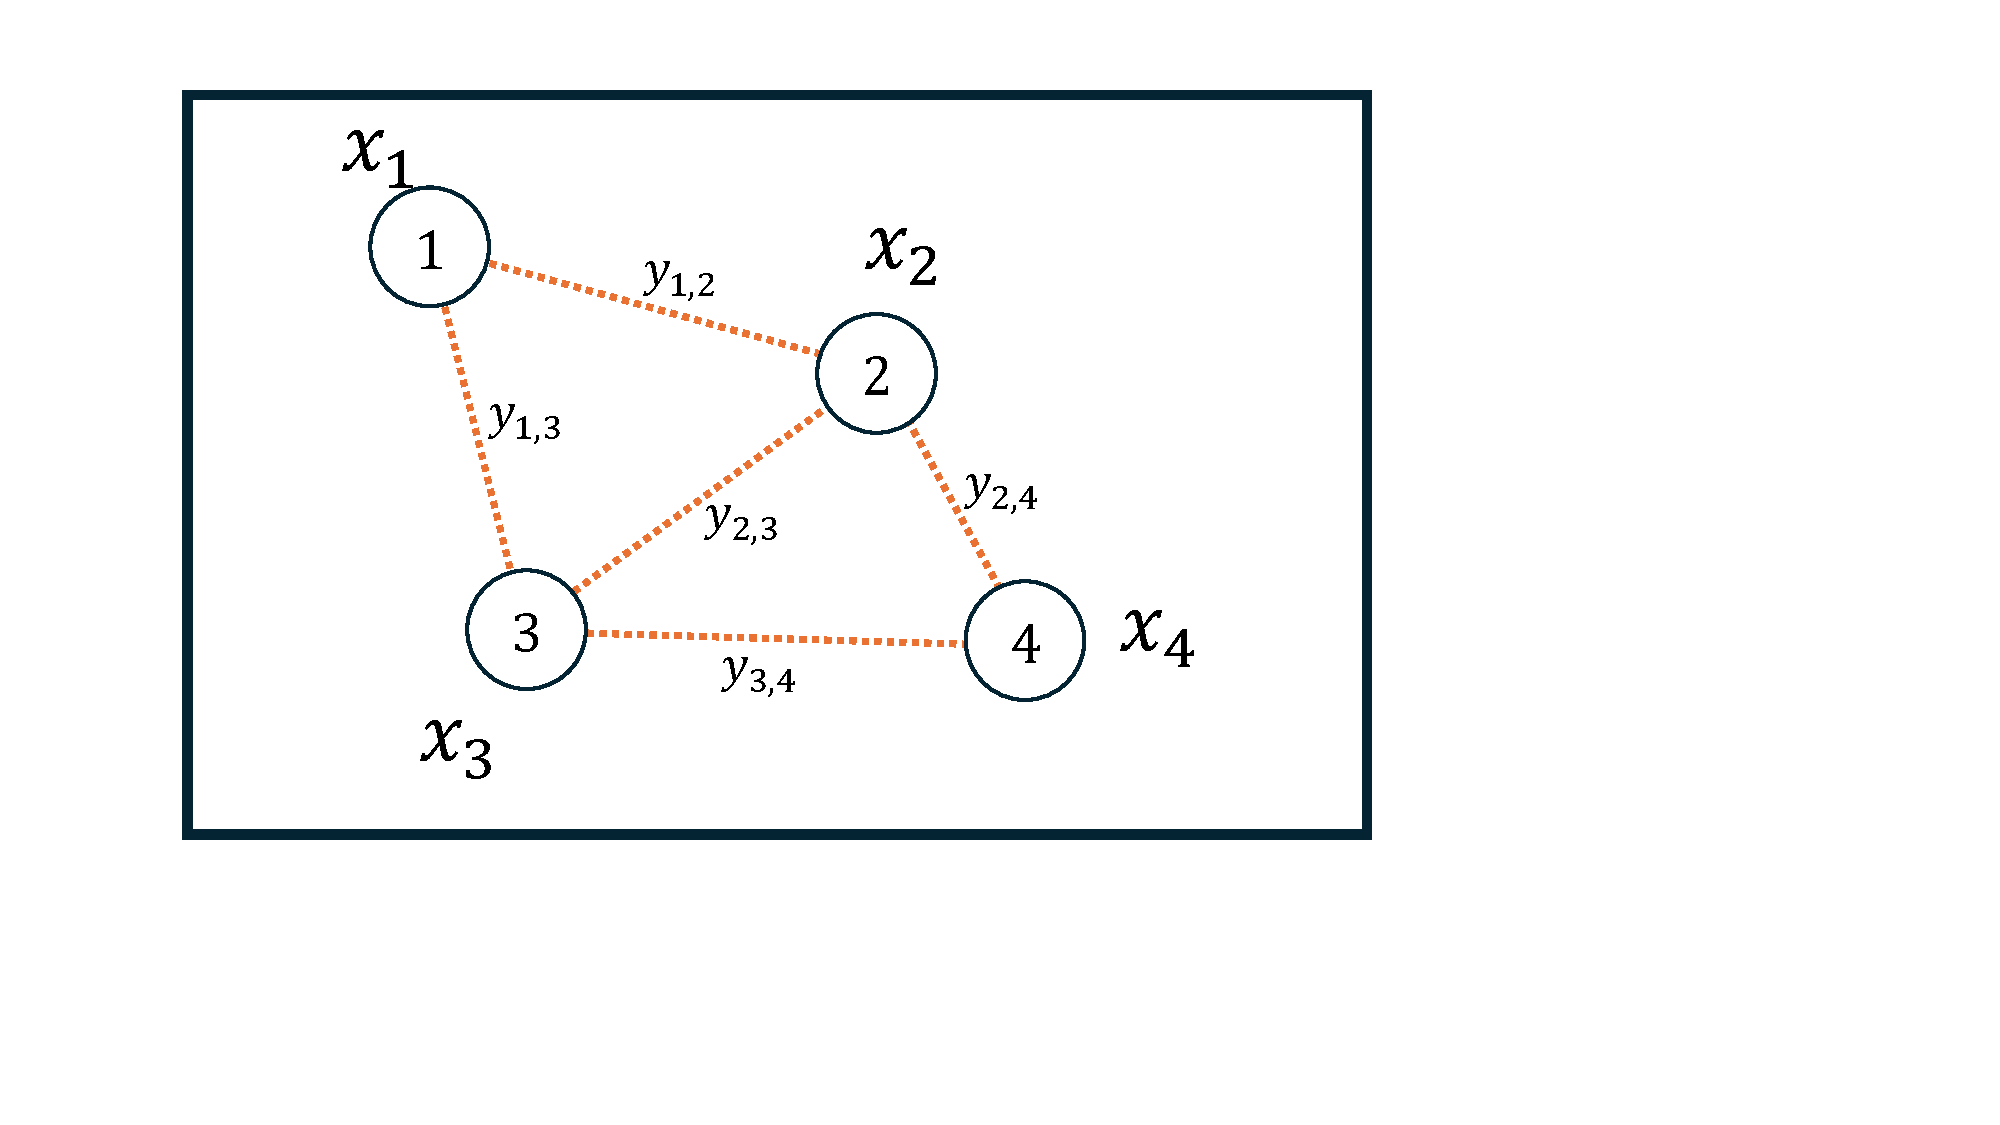
\includegraphics[width=\linewidth,trim=31mm 48mm 106mm 15mm, clip]{graph.pdf}
    \caption{Problem reformulation. In the figure, we have a graph $\mathcal{G}=(\mathcal{V}, \mathcal{E})$ where the directed edges $(i, j) \in \mathcal{E}$ have weights $l_{i,j}$ and the vertices $k \in \mathcal{V}$ have positions $x^{(k)}_t$.}
    \label{fig:problem-graph} 
\end{figure}
As described in section~\ref{sec:lit-rev}, this is a non-convex with no known efficient global solver. However, the Riemannian Elevator~\cite{R_elevator} provides an approximate solution as well as a non-trivial lower bound on the problem which we can use to determine the quality of the solution. Given this, we can approximately solve the localization problem for the initial positions. The estimates can be further refined using gradient descent on the stress minimization problem as described in previous sections. 

We use the notation defined in table~\ref{tab:notation} below to describe the graph and the data collected from it.
\FloatBarrier
\begin{table}[ht]
    \centering
    \caption{Additional definitions}
    \label{tab:notation}
    \begin{tabularx}{\linewidth}{lX}
        $\mathbf{J}_t \in \R{m \times 2}$ & 
        \textit{Connectivity matrix}.  Each row $(i, j)\in\mathcal{E}$ represents a directed edge of the graph. \\
        $\mathbf{y}_t \in \R{m}$ & 
        \textit{Measurement vector}. Each row $k$ is the distance measurement between the two nodes at row $k$ in $\mathbf{J}_t$. \\
        $\bm{\psi}_t \in \R{m}$ &
        \textit{Noise variance vector}. Each row $k$ is the variance of the noise measurement at row $k$ in $\mathbf{y}_t$. 
    \end{tabularx}
\end{table}

\subsection{Coordinate System}
Any solution to the stress minimization problem, either local or global is not unique. Since the stress function is invariant under translation, rotation, and mirroring, there is no way to determine a coordinate system matching some world coordinates. Therefore, any chosen coordinate system is as valid as any other. Initially, the Riemannian elevator is used to get estimates of the positions of the robots. This initial guess gives us the coordinate system to use in future time steps. However, when tracking the positions over longer a longer time horizon, it probable that the coordinate system will begin to drift. This means that, even though a point may have the same coordinates at two different time steps, $x^{(i)}_t = x^{(i)}_\tau$ for $t \neq \tau$, the real robot might not be at the same position at those two time steps. This is a fundamental limitation of the problem setup, as there is no measurements of the outside world. To remedy this, outside anchors could be provided which would both give a reference coordinate frame, as well as enable other localization algorithms like traditional SLAM. 

Ultimately, these are issues innate to the chosen problem, and even if the relative localization problem was solved globally, they would still persist. As such, we make no effort to solve these as the relative localization problem remains interesting regardless of limitations.

% \subsection{Unbiased Coordinates}
% Solving the localization problem, be it through the Riemannian Elevator or through stress minimization, is not enough. Since the stress function is invariant under translation, rotation, and mirroring, we need some canonical way of representing coordinates. For this, we use the mean and the SVD of the point list.

% Given a minimum of the stress function at a time $t$
% \begin{align}
%     \mathbf{X}_t = \begin{bmatrix}
%         (\x[1])^\top \\ \vdots \\ (\x[n])^\top
%     \end{bmatrix}
% \end{align}
% we subtract the mean from each point to get the same set of points centered at the origin.
% \begin{align}
%     \tilde{\mathbf{X}}_t = \begin{bmatrix}
%         (\x[1])^\top - \mu_{x_t}^\top \\ \vdots \\ (\x[n])^\top - \mu_{x_t}^\top
%     \end{bmatrix}
% \end{align}
% To cancel out rotation we determine the SVD and get 
% \begin{align}
%     U_t &\in \R{m \times 2} \\
%     \Sigma_t &\in \R{2 \times 2} \\
%     V_t &\in \R{2 \times 2}
% \end{align}
% Assuming that the two singular values are distinct, this is unique up to scaling by $\pm 1$ on the columns of $U_t$ and $V_t$. If we interpret $V_t$ as a basis for the 

% This means that the matrix 
% \begin{align}
%     U_t \Sigma_t V_t^\top V_t = U_t \Sigma_t
% \end{align}

\subsection{Algorithm Description}
With the content in previous sections, we can now define algorithm~\ref{algo:estimation}, the online estimation algorithm. For conciseness, we define the function $\text{RE}(C, \tilde{D}, W)$ the output of the Riemannian elevator, and $\text{KA}(\hat{\mathbf{x}}_{t \mid t-1}, \mathbf{y}_t, \bm{\psi}_t)$ as the output of gradient descent using Kruskal's algorithm. 



\begin{algorithm}
    \caption{Online estimation}\label{algo:estimation}
    \textbf{Inputs:} Connectivity matrix $\mathbf{J}_0$, measurement vector $\mathbf{y}_0$, noise power vector $\bm{\psi}_0$
    
    \textbf{Initialize:} Get an initial guess
    \begingroup\setstretch{1.2} % Increase line spacing
    \begin{algorithmic}[1]
        \Statex \underline{Find initial guess with Riemannian elevator}
        \State Construct matrices $C$, $\tilde{D}$, and $W$, see \cite{R_elevator}
        \State $\hat{\mathbf{X}}_0 \ \leftarrow\ \text{RE}(C, \tilde{D}, W)$
        \State Recover $\hat{\mathbf{x}}_{0 \mid 0} \in \R{3n}$ from $\hat{\mathbf{X}}_0 \in \R{n \times 2}$, assuming $\hat{\theta}^{(i)} = 0$ with high uncertainty.
    \end{algorithmic}

    \textbf{Track:} Continuously track the states
    \begin{algorithmic}[1]
        \Statex \underline{Predict}
        \State $\hat{\mathbf{x}}_{t \mid t-1} = \mathbf{f}(\hat{\mathbf{x}}_{t-1 \mid t-1}, \mathbf{u}_{t-1})$
        \State $\mathbf{P}_{t \mid t-1} = \mathbf{F}_t \mathbf{P}_{t-1 \mid t-1} \mathbf{F}_t^\top + \mathbf{Q}_t$
        \Statex \underline{Measure}
        \State Collect distance measurements $\mathbf{y}_t$
        \State Get position measurements $\mathbf{z}_t = \text{KA}(\hat{\mathbf{x}}_{t \mid t-1}, \mathbf{y}_t, \bm{\psi}_t)$ and corresponding matrices and vectors $\mathbf{J}_t$, $\mathbf{L}_t$, $\bm{\psi}_t$
        \Statex \underline{Update}
        \State $\mathbf{K}_t = \mathbf{P}_{t \mid t-1} \mathbf{H}^\top_t (\mathbf{H}_t \mathbf{P}_{t \mid t-1} \mathbf{H}_t^\top + \mathbf{R}_t)^{-1}$
        \State $\hat{\mathbf{x}}_{t \mid t} = \hat{\mathbf{x}}_{t\mid t-1} + \mathbf{K}_t (\mathbf{z}_t - \mathbf{g}(\hat{\mathbf{x}}_{t \mid t-1}))$
        \State $\mathbf{P}_{t \mid t} = (\mathbf{I} - \mathbf{K}_t \mathbf{H}_t) \mathbf{P}_{t \mid t-1}$
        \Statex \underline{Repeat}: Go to \underline{Predict}
    \end{algorithmic}
    \endgroup
\end{algorithm}